\chapter{Data Flow Testing}
Data flow testing tries to identify flow anomalies based on the associations between values and variables. It uses the control flow graph to explore the anomalies. Examples of the anomalies include the usage of uninitialized variables and initialized variables are not used at all.

If a value is bound to a variable, then we call it as a \emph{definition} of the variable. On the other hand, if the bound value is referred to in the program, we call it as a \emph{use} of the variable. If a variable is used inside a predicate and has the right to decide about the execution path, then the type of use is called \emph{predicate use (p-use)}. Similarly, if a variable's value is used to compute another variables value, we call it as \emph{computation use (c-use)}.

\section{Data Flow Graph}
Data flow graphs (an example is shown in Figure \ref{fig:data-flow-graph}) are generally produced by the special language translators instead of developers. The main objective of data flow graphs are to mark the definitions and uses of variables that are used inside of the program. A data flow graph is a directed graph and constructed as follows:
\begin{itemize}[noitemsep]
    \item A sequence of definitions and c-uses is associated with each node of the graph.
    \item A set of p-uses is associated with each edge of the graph.
    \item The entry node has a definition of each parameter and each non-local variable which occurs in the subprogram.
    \item The exit node has an undefinition of each local variable.
\end{itemize}

\begin{figure}[H]
    \centering
    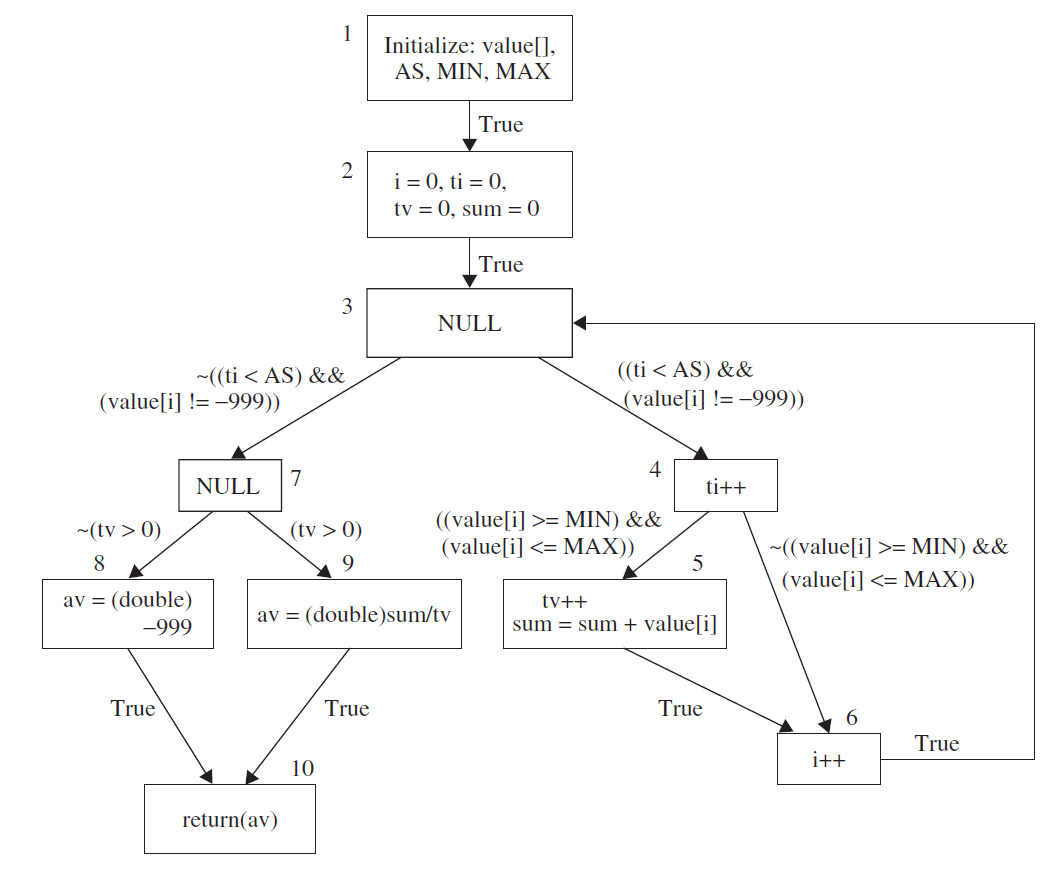
\includegraphics[width=0.5\textwidth]{images/data-flow-graph.png}
    \caption{Data flow graph example.}
    \label{fig:data-flow-graph}
\end{figure}

\section{Exercises}
Given the following exercises. Fill the tables below according to the given examples using the code snippets of the exercises.

\begin{exercise}
    ReturnAverage function computes the average of all those numbers in the input array in the positive range [MIN, MAX]. The maximum size of the array is AS. But, the array size could be smaller than AS in which case the end of input is represented by -999.
    
    \begin{lstlisting}[caption={A program to calculate a ranged average in a list.}]
public double returnAverage (int value[], int AS, int MIN, int MAX) {
    /*
     * Function: ReturnAverage Computes the average of all those numbers in the
     * input array in the positive range [MIN, MAX]. The maximum size of the array
     * is AS. The array size could be smaller than AS in which case the end of
     * input is represented by -999.
     */

    int i, ti, tv, sum;
    double av;
    i = 0;
    ti = 0;
    tv = 0;
    sum = 0;
    while (ti < AS && value[i] != -999) {
        ti++;
        if (value[i] >= MIN && value[i] <= MAX) {
            tv++;
            sum = sum + value[i];
        }
        i++; //i=i+1
    }
    if (tv > 0)
        av = (double) sum / tv;
    else
        av = (double) -999;
    return (av);
}
    \end{lstlisting}
    
    \begin{table}[H]
        \centering
        \renewcommand{\arraystretch}{1.2}
        \caption{Def-Use pairs and related test cases.}
        \label{tab:e9-answer-table}
        \begin{adjustbox}{max width=\textwidth}
            \begin{tabular}{|l|l|l|l|l|l|}
                \toprule
                \thead{Variable} & \thead{Definition line} & \thead{Use line} & \thead{Def-Use pair} & \thead{Feasibility} & \thead{Test case}\\
                \midrule
                \lstinline!value[]! & 1 & 15 (Predicate) & 1-15 & \cmark & \makecell{value[] not empty\\AS = 8, MIN = 9, MAX = 50}\\
                \lstinline!value[]! & 1 & 17 (Predicate) & 1-17 & \cmark & MIN <= value[i] <= MAX\\
                \lstinline!value[]! & 1 & 19 (Comp.) & 1-19 & \cmark & MIN <= value[i] <= MAX\\
                \lstinline!tv! & 11 & 18 & 18-25 & \xmark & tv increments here, cannot be 0\\
                 & & & & & \\
                 & & & & & \\
                 & & & & & \\
                 & & & & & \\
                 & & & & & \\
                 & & & & & \\
                 & & & & & \\
                 & & & & & \\
                 & & & & & \\
                 & & & & & \\
                 & & & & & \\
                 & & & & & \\
                 & & & & & \\
                 & & & & & \\
                 & & & & & \\
                 & & & & & \\
                 & & & & & \\
                 & & & & & \\
                 & & & & & \\
                 & & & & & \\
                 & & & & & \\
                 & & & & & \\
                 & & & & & \\
                 & & & & & \\
                 & & & & & \\
                 & & & & & \\
                 & & & & & \\
                 & & & & & \\
                 & & & & & \\
                 & & & & & \\
                 & & & & & \\
                 & & & & & \\
                 & & & & & \\
                 & & & & & \\
                 & & & & & \\
                 & & & & & \\
                \bottomrule
            \end{tabular}
        \end{adjustbox}
    \end{table}
\end{exercise}

\begin{solution}
    Some of the answers for the exercise are given in the table below.
    
    \begin{table}[H]
        \centering
        \renewcommand{\arraystretch}{1.2}
        \caption{Def-Use pairs and related test cases.}
        \label{tab:e9-answers}
        \begin{adjustbox}{max width=\textwidth}
            \begin{tabular}{|l|l|l|l|l|c|}
                \toprule
                \thead{Variable} & \thead{Definition line} & \thead{Use line} & \thead{Def-Use pair} & \thead{Feasibility} & \thead{Test case}\\
                \midrule
                \lstinline!value[]! & 1 & 15 (Predicate) & 1-15 & \cmark & \makecell{value[] not empty\\AS = 8, MIN = 9, MAX = 50}\\
                \lstinline!value[]! & 1 & 17 (Predicate) & 1-17 & \cmark & MIN <= value[i] <= MAX\\
                \lstinline!value[]! & 1 & 19 (Comp.) & 1-19 & \cmark & MIN <= value[i] <= MAX\\
                \lstinline!tv! & 11 & 18 & 18-25 & \xmark & tv increments here, cannot be 0\\
                \lstinline!AS! & 1 & 15 (Predicate) & 1-15 & \cmark & everyting\\
                \lstinline!MIN! & 1 & 17 (Predicate) & 1-17 & \cmark & \makecell{AS > 0\\value[] not empty}\\
                \lstinline!MAX! & 1 & 17 (Predicate) & 1-17 & \cmark & \makecell{AS > 0\\value[] not empty\\value[0]=3, MIN=1}\\
                \lstinline!i! & 11 & 15 & 11-15 & \cmark & AS > 0\\
                \lstinline!i! & 11 & 17 & 11-17 & \cmark & \makecell{AS>0, value[] not empty\\value[0]=2\\MIN=3}\\
                \lstinline!i! & 11 & 17 & 11-17 & \cmark & \makecell{AS>0, value[] not empty\\value[0]=3\\MIN=2}\\
                \lstinline!i! & 11 & 19 & 11-19 & \cmark & \makecell{AS>0, value[] not empty\\value[0]=3\\MIN=2\\MAX=5}\\
                \lstinline!i! & 11 & 21 & 11-21 & \cmark & \makecell{value[] not empty\\AS = 8, MIN = 9, MAX = 50}\\
                \bottomrule
            \end{tabular}
        \end{adjustbox}
    \end{table}
\end{solution}